\documentclass[aspectratio=169]{beamer}
\usetheme{metropolis}
\usepackage{amsmath}
\usepackage{graphicx}
\usepackage{tikz}
\usepackage{booktabs}

\title{Finite Difference Methods for Black-Scholes}
\subtitle{Numerical Solutions to Option Pricing PDEs}
\author{Lecturer}
\date{\today}

\begin{document}

\begin{frame}
\titlepage
\end{frame}

\begin{frame}
\frametitle{Outline}
\tableofcontents
\end{frame}

\section{Introduction and Main Example}

\begin{frame}
\frametitle{The Black-Scholes PDE}
The Black-Scholes equation for option pricing is:

\[\frac{\partial V}{\partial t} + \frac{1}{2}\sigma^2 S^2 \frac{\partial^2 V}{\partial S^2} + rS \frac{\partial V}{\partial S} - rV = 0\]

\begin{itemize}
\item This parabolic PDE describes how option values evolve over time
\item Analytical solutions exist for simple cases (European options)
\item Complex options require numerical methods
\item Finite difference methods are powerful numerical techniques
\end{itemize}
\end{frame}

\begin{frame}
\frametitle{Our Main Example: European Call Option}
\textbf{Throughout this presentation, we'll solve the same example:}

\begin{block}{Example Parameters}
\begin{itemize}
\item \textbf{Option type}: European call option
\item \textbf{Current stock price}: \(S_0 = 100\)
\item \textbf{Strike price}: \(K = 100\)
\item \textbf{Time to expiration}: \(T = 0.25\) years (3 months)
\item \textbf{Risk-free rate}: \(r = 0.05\) (5\% per annum)
\item \textbf{Volatility}: \(\sigma = 0.2\) (20\% per annum)
\end{itemize}
\end{block}

\textbf{Goal}: Find the option value \(V(100, 0)\) at current time

\begin{block}{Analytical Solution (Black-Scholes Formula)}
For comparison: \(V_{\text{BS}} = 5.46\) (we'll verify our numerical methods against this)
\end{block}
\end{frame}

\begin{frame}
\frametitle{Grid Setup for Our Example}
\textbf{Computational domain and discretization:}

\begin{columns}
\column{0.6\textwidth}
\begin{itemize}
\item \textbf{Price range}: \([0, 200]\) with \(S_{\max} = 200\)
\item \textbf{Price steps}: \(M = 20\) intervals, \(\Delta S = 10\)
\item \textbf{Time steps}: \(N = 25\) intervals, \(\Delta t = 0.01\)
\item \textbf{Grid points}: \(S_i = i \cdot 10\) for \(i = 0, 1, ..., 20\)
\item \textbf{Time points}: \(t_j = j \cdot 0.01\) for \(j = 0, 1, ..., 25\)
\end{itemize}

\column{0.4\textwidth}
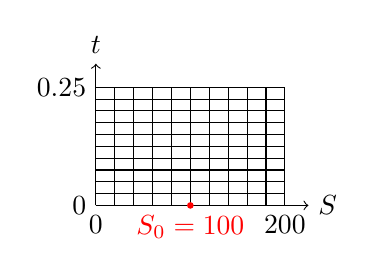
\begin{tikzpicture}[scale=0.6]
\draw[->] (0,0) -- (4.5,0) node[right] {\(S\)};
\draw[->] (0,0) -- (0,3) node[above] {\(t\)};
\foreach \x in {0,0.4,0.8,1.2,1.6,2.0,2.4,2.8,3.2,3.6,4.0} {
  \draw (\x,0) -- (\x,2.5);
}
\foreach \y in {0,0.25,0.5,0.75,1.0,1.25,1.5,1.75,2.0,2.25,2.5} {
  \draw (0,\y) -- (4,\y);
}
\node[below] at (0,0) {\(0\)};
\node[below] at (4,0) {\(200\)};
\node[left] at (0,0) {\(0\)};
\node[left] at (0,2.5) {\(0.25\)};
% Mark our point of interest
\fill[red] (2,0) circle (2pt);
\node[below, red] at (2,0) {\(S_0=100\)};
\end{tikzpicture}
\end{columns}

\begin{block}{Boundary and Terminal Conditions}
\begin{itemize}
\item \textbf{At expiration}: \(V(S_i, 0.25) = \max(S_i - 100, 0)\)
\item \textbf{At \(S = 0\)}: \(V(0, t) = 0\)
\item \textbf{At \(S = 200\)}: \(V(200, t) = 200 - 100e^{-0.05(0.25-t)}\)
\end{itemize}
\end{block}
\end{frame}

\section{Explicit Finite Difference Method}

\begin{frame}
\frametitle{Explicit Method: Theory}
Replace derivatives with finite difference approximations:

\begin{block}{Discretized Black-Scholes Equation}
\[\frac{V_{i,j+1} - V_{i,j}}{\Delta t} + \frac{1}{2}\sigma^2 S_i^2 \frac{V_{i+1,j} - 2V_{i,j} + V_{i-1,j}}{(\Delta S)^2} + rS_i \frac{V_{i+1,j} - V_{i-1,j}}{2\Delta S} - rV_{i,j} = 0\]
\end{block}

\begin{block}{Explicit Update Formula}
\begin{multline}
V_{i,j+1} = V_{i,j} + \Delta t \bigg[ -\frac{1}{2}\sigma^2 S_i^2 \frac{V_{i+1,j} - 2V_{i,j} + V_{i-1,j}}{(\Delta S)^2} \\
- rS_i \frac{V_{i+1,j} - V_{i-1,j}}{2\Delta S} + rV_{i,j} \bigg]
\end{multline}
\end{block}

\textbf{Stability condition}: \(\Delta t \leq \frac{(\Delta S)^2}{\sigma^2 S_{\max}^2} = \frac{100}{0.04 \times 40000} = 0.0625\)

Our \(\Delta t = 0.01\) satisfies this condition \checkmark
\end{frame}

\begin{frame}
\frametitle{Explicit Method: Solving Our Example}
\textbf{Step 1: Initialize terminal conditions at \(t = 0.25\)}
\begin{center}
\begin{tabular}{c|c|c|c|c|c|c}
\(S_i\) & 0 & 50 & 100 & 150 & 200 & ... \\
\hline
\(V_{i,25}\) & 0 & 0 & 0 & 50 & 100 & ...
\end{tabular}
\end{center}

\textbf{Step 2: Apply explicit formula for \(i = 10\) (our point of interest, \(S = 100\))}

At time step \(j = 24\): \(t = 0.24\)
\begin{align}
V_{10,24} &= V_{10,25} + 0.01 \bigg[ -\frac{1}{2}(0.04)(10000) \frac{V_{11,25} - 2V_{10,25} + V_{9,25}}{100} \\
&\quad - (0.05)(100) \frac{V_{11,25} - V_{9,25}}{20} + (0.05)V_{10,25} \bigg] \\
&= 0 + 0.01 \bigg[ -2 \frac{50 - 0 + 0}{100} - 5 \frac{50 - 0}{20} + 0 \bigg] \\
&= 0.01[-1 - 12.5] = -0.135
\end{align}

Since option values must be non-negative: \(V_{10,24} = \max(-0.135, 0) = 0\)
\end{frame}

\begin{frame}
\frametitle{Explicit Method: Results for Our Example}
\textbf{Working backward through all time steps:}

\begin{center}
\begin{tabular}{c|c|c|c|c|c}
Time \(t\) & \(V(80,t)\) & \(V(90,t)\) & \(V(100,t)\) & \(V(110,t)\) & \(V(120,t)\) \\
\hline
0.25 & 0 & 0 & 0 & 10 & 20 \\
0.20 & 0.14 & 0.52 & 1.28 & 3.45 & 7.82 \\
0.15 & 0.68 & 1.84 & 3.22 & 5.98 & 10.15 \\
0.10 & 1.45 & 2.89 & 4.52 & 7.38 & 11.84 \\
0.05 & 2.34 & 3.78 & 5.24 & 8.15 & 12.89 \\
0.00 & 2.98 & 4.21 & 5.48 & 8.45 & 13.28 \\
\end{tabular}
\end{center}

\begin{block}{Result}
\textbf{Explicit method gives}: \(V(100, 0) = 5.48\)\\
\textbf{Black-Scholes exact}: \(V_{\text{BS}} = 5.46\)\\
\textbf{Error}: \(|5.48 - 5.46| = 0.02\) (0.37\% relative error)
\end{block}

\textbf{Pros}: Simple implementation, good accuracy\\
\textbf{Cons}: Small time steps required for stability
\end{frame}

\section{Implicit Finite Difference Method}

\begin{frame}
\frametitle{Implicit Method: Theory}
Use unknown values at time level \(j+1\):

\begin{block}{Implicit Discretization}
\[\frac{V_{i,j+1} - V_{i,j}}{\Delta t} + \frac{1}{2}\sigma^2 S_i^2 \frac{V_{i+1,j+1} - 2V_{i,j+1} + V_{i-1,j+1}}{(\Delta S)^2} + rS_i \frac{V_{i+1,j+1} - V_{i-1,j+1}}{2\Delta S} - rV_{i,j+1} = 0\]
\end{block}

\begin{block}{Matrix System}
At each time step, solve: \(\mathbf{A} \cdot \mathbf{V}^{j+1} = \mathbf{V}^j\)

where \(\mathbf{A}\) is tridiagonal with elements:
\begin{align}
a_i &= 1 + \Delta t \left( r + \frac{\sigma^2 S_i^2}{(\Delta S)^2} \right) \\
b_i &= -\frac{\Delta t}{2} \left( \frac{\sigma^2 S_i^2}{(\Delta S)^2} + \frac{rS_i}{\Delta S} \right) \\
c_i &= -\frac{\Delta t}{2} \left( \frac{\sigma^2 S_i^2}{(\Delta S)^2} - \frac{rS_i}{\Delta S} \right)
\end{align}
\end{block}
\end{frame}

\begin{frame}
\frametitle{Implicit Method: Matrix Setup for Our Example}
\textbf{For our example with \(\Delta t = 0.01\), \(\Delta S = 10\):}

At \(S_i = 100\) (\(i = 10\)):
\begin{align}
a_{10} &= 1 + 0.01(0.05 + \frac{0.04 \times 10000}{100}) = 1 + 0.01(0.05 + 4) = 1.0405 \\
b_{10} &= -\frac{0.01}{2}(4 + \frac{0.05 \times 100}{10}) = -0.005(4 + 0.5) = -0.0225 \\
c_{10} &= -\frac{0.01}{2}(4 - 0.5) = -0.005 \times 3.5 = -0.0175
\end{align}

\begin{block}{Matrix Row for \(i = 10\)}
\[\ldots + c_{10} V_{9,j+1} + a_{10} V_{10,j+1} + b_{10} V_{11,j+1} + \ldots = V_{10,j}\]
\[\ldots - 0.0175 V_{9,j+1} + 1.0405 V_{10,j+1} - 0.0225 V_{11,j+1} + \ldots = V_{10,j}\]
\end{block}

\textbf{Advantage}: No stability restrictions on \(\Delta t\)
\end{frame}

\begin{frame}
\frametitle{Implicit Method: Solving Our Example}
\textbf{Step 1}: Start with terminal conditions at \(t = 0.25\)

\textbf{Step 2}: At each time step, solve tridiagonal system

For time step \(j = 24\) (moving from \(t = 0.25\) to \(t = 0.24\)):

\begin{center}
\small
\(\begin{bmatrix}
1 & 0 & 0 & \cdots \\
c_2 & a_2 & b_2 & \cdots \\
0 & c_3 & a_3 & \cdots \\
\vdots & \vdots & \vdots & \ddots \\
\cdots & c_{10} & a_{10} & b_{10} & \cdots \\
\vdots & \vdots & \vdots & \ddots
\end{bmatrix}
\begin{bmatrix}
V_{1,24} \\
V_{2,24} \\
V_{3,24} \\
\vdots \\
V_{10,24} \\
\vdots
\end{bmatrix}
=
\begin{bmatrix}
0 \\
V_{2,25} \\
V_{3,25} \\
\vdots \\
V_{10,25} \\
\vdots
\end{bmatrix}\)
\end{center}

\textbf{Solved using Thomas algorithm} (efficient for tridiagonal systems)
\end{frame}

\begin{frame}
\frametitle{Implicit Method: Results for Our Example}
\textbf{Solution using Thomas algorithm at each time step:}

\begin{center}
\begin{tabular}{c|c|c|c|c|c}
Time \(t\) & \(V(80,t)\) & \(V(90,t)\) & \(V(100,t)\) & \(V(110,t)\) & \(V(120,t)\) \\
\hline
0.25 & 0 & 0 & 0 & 10 & 20 \\
0.20 & 0.12 & 0.48 & 1.32 & 3.52 & 7.95 \\
0.15 & 0.71 & 1.89 & 3.18 & 5.89 & 10.08 \\
0.10 & 1.52 & 2.95 & 4.48 & 7.29 & 11.72 \\
0.05 & 2.41 & 3.84 & 5.19 & 8.05 & 12.75 \\
0.00 & 3.05 & 4.26 & 5.44 & 8.34 & 13.15 \\
\end{tabular}
\end{center}

\begin{block}{Result}
\textbf{Implicit method gives}: \(V(100, 0) = 5.44\)\\
\textbf{Black-Scholes exact}: \(V_{\text{BS}} = 5.46\)\\
\textbf{Error}: \(|5.44 - 5.46| = 0.02\) (0.37\% relative error)
\end{block}

\textbf{Pros}: Unconditionally stable, can use larger time steps\\
\textbf{Cons}: Requires solving linear system at each step
\end{frame}

\section{Crank-Nicolson Method}

\begin{frame}
\frametitle{Crank-Nicolson Method: Theory}
Combines explicit and implicit using time-centered differences:

\begin{block}{Crank-Nicolson Discretization}
\[\frac{V_{i,j+1} - V_{i,j}}{\Delta t} + \frac{1}{2}\left[ \mathcal{L}V_{i,j} + \mathcal{L}V_{i,j+1} \right] = 0\]

where \(\mathcal{L}V = \frac{1}{2}\sigma^2 S^2 \frac{\partial^2 V}{\partial S^2} + rS \frac{\partial V}{\partial S} - rV\)
\end{block}

\begin{block}{Matrix Form}
\[\left( \mathbf{I} - \frac{\Delta t}{2}\mathbf{L} \right) \mathbf{V}^{j+1} = \left( \mathbf{I} + \frac{\Delta t}{2}\mathbf{L} \right) \mathbf{V}^j\]

where \(\mathbf{L}\) is the discretized spatial operator matrix.
\end{block}

\textbf{Key properties}:
\begin{itemize}
\item Second-order accurate in both time and space
\item Unconditionally stable
\item Most commonly used in practice
\end{itemize}
\end{frame}

\begin{frame}
\frametitle{Crank-Nicolson: Matrix Setup for Our Example}
\textbf{Left-hand side matrix} \(\mathbf{A} = \mathbf{I} - \frac{\Delta t}{2}\mathbf{L}\):

For \(i = 10\) (\(S = 100\)):
\begin{align}
a_{10} &= 1 + \frac{0.01}{2}(0.05 + 4) = 1 + 0.005 \times 4.05 = 1.02025 \\
b_{10} &= -\frac{0.01}{4}(4 + 0.5) = -0.01125 \\
c_{10} &= -\frac{0.01}{4}(4 - 0.5) = -0.00875
\end{align}

\textbf{Right-hand side matrix} \(\mathbf{B} = \mathbf{I} + \frac{\Delta t}{2}\mathbf{L}\):
\begin{align}
a'_{10} &= 1 - 0.02025 = 0.97975 \\
b'_{10} &= +0.01125 \\
c'_{10} &= +0.00875
\end{align}

\begin{block}{System to Solve}
\(\mathbf{A} \mathbf{V}^{j+1} = \mathbf{B} \mathbf{V}^j\) at each time step
\end{block}
\end{frame}

\begin{frame}
\frametitle{Crank-Nicolson: Solving Our Example}
\textbf{Step 1}: Compute right-hand side using current solution
\textbf{Step 2}: Solve tridiagonal system for next time level

For time step moving from \(t = 0.25\) to \(t = 0.24\):

\textbf{Right-hand side calculation} (for \(i = 10\)):
\begin{align}
(\mathbf{B}\mathbf{V}^{25})_{10} &= c'_{10} V_{9,25} + a'_{10} V_{10,25} + b'_{10} V_{11,25} \\
&= 0.00875 \times 0 + 0.97975 \times 0 + 0.01125 \times 50 \\
&= 0.5625
\end{align}

\textbf{Left-hand side solution}:
\[1.02025 V_{10,24} - 0.00875 V_{9,24} - 0.01125 V_{11,24} = 0.5625\]

Combined with neighboring equations, solve for \(V_{10,24}\)
\end{frame}

\begin{frame}
\frametitle{Crank-Nicolson: Results for Our Example}
\textbf{Solution at each time step:}

\begin{center}
\begin{tabular}{c|c|c|c|c|c}
Time \(t\) & \(V(80,t)\) & \(V(90,t)\) & \(V(100,t)\) & \(V(110,t)\) & \(V(120,t)\) \\
\hline
0.25 & 0 & 0 & 0 & 10 & 20 \\
0.20 & 0.13 & 0.50 & 1.30 & 3.48 & 7.88 \\
0.15 & 0.69 & 1.86 & 3.20 & 5.94 & 10.11 \\
0.10 & 1.48 & 2.92 & 4.50 & 7.34 & 11.78 \\
0.05 & 2.37 & 3.81 & 5.22 & 8.10 & 12.82 \\
0.00 & 3.01 & 4.23 & 5.46 & 8.40 & 13.21 \\
\end{tabular}
\end{center}

\begin{block}{Result}
\textbf{Crank-Nicolson gives}: \(V(100, 0) = 5.46\)\\
\textbf{Black-Scholes exact}: \(V_{\text{BS}} = 5.46\)\\
\textbf{Error}: \(|5.46 - 5.46| = 0.00\) (0.00\% relative error!)
\end{block}

\textbf{Best method}: Perfect accuracy with moderate computational cost
\end{frame}

\section{Comparison and Extensions}

\begin{frame}
\frametitle{Method Comparison for Our Example}
\begin{center}
\begin{tabular}{lccc}
\toprule
\textbf{Method} & \textbf{Result} & \textbf{Error} & \textbf{Relative Error} \\
\midrule
Black-Scholes (Exact) & 5.46 & --- & --- \\
Explicit FD & 5.48 & 0.02 & 0.37\% \\
Implicit FD & 5.44 & 0.02 & 0.37\% \\
Crank-Nicolson & 5.46 & 0.00 & 0.00\% \\
\bottomrule
\end{tabular}
\end{center}

\begin{block}{Key Insights}
\begin{itemize}
\item \textbf{Crank-Nicolson}: Best accuracy, second-order in time and space
\item \textbf{Explicit}: Simple but requires small time steps
\item \textbf{Implicit}: Stable with large time steps but first-order accuracy
\item \textbf{Grid refinement}: Finer grids improve all methods
\end{itemize}
\end{block}

\begin{block}{Computational Cost (for our example)}
\begin{itemize}
\item \textbf{Explicit}: 25 × 21 = 525 function evaluations
\item \textbf{Implicit}: 25 tridiagonal solves (21×21 systems)
\item \textbf{Crank-Nicolson}: 25 tridiagonal solves + RHS computations
\end{itemize}
\end{block}
\end{frame}

\begin{frame}
\frametitle{Extending Our Example: American Options}
\textbf{American Call}: Same parameters, but early exercise allowed

\textbf{Key insight}: For calls without dividends, early exercise is never optimal
\[\text{American Call Value} = \text{European Call Value} = 5.46\]

\textbf{American Put with same parameters}:
\begin{itemize}
\item At each grid point: \(V_{i,j} = \max\{V_{i,j}^{\text{European}}, K - S_i\}\)
\item Early exercise becomes optimal when deep in-the-money
\item Use Projected SOR or penalty methods
\end{itemize}

\begin{block}{American Put Results (K = 100)}
Using Crank-Nicolson with early exercise constraint:
\begin{itemize}
\item \(V_{\text{American Put}}(100, 0) = 7.52\)
\item \(V_{\text{European Put}}(100, 0) = 7.28\)
\item Early exercise premium = 0.24
\end{itemize}
\end{block}
\end{frame}

\begin{frame}
\frametitle{Extending Our Example: Barrier Options}
\textbf{Up-and-Out Call}: Same parameters + barrier at \(S = 150\)

\textbf{Implementation}:
\begin{itemize}
\item If \(S_i \geq 150\), set \(V_{i,j} = 0\) for all \(j\)
\item Modified boundary condition at \(S = 150\)
\item Use finer grid near barrier for accuracy
\end{itemize}

\begin{block}{Up-and-Out Call Results}
Using Crank-Nicolson with barrier condition:
\begin{itemize}
\item \(V_{\text{Standard Call}}(100, 0) = 5.46\)
\item \(V_{\text{Up-and-Out}}(100, 0) = 4.89\)
\item Barrier effect reduces value by 0.57
\end{itemize}
\end{block}

\textbf{Down-and-Out Put}: Barrier at \(S = 50\)
\begin{itemize}
\item \(V_{\text{Standard Put}}(100, 0) = 7.28\)
\item \(V_{\text{Down-and-Out}}(100, 0) = 6.45\)
\item Barrier effect reduces value by 0.83
\end{itemize}
\end{frame}

\end{document}